
\documentclass[oneside]{ausarbeitung}
\bibliography{latexlit.bib}


% ----------------------------------------------------------------------

\begin{document}

%--- Sprachauswahl
% Erlaubte Werte:
%   \selectlanguage{english}
%   \selectlanguage{ngerman}
\selectlanguage{ngerman}

%--- Art der Arbeit
% Erlaubte Werte:
%   \Praxissemesterbericht
%   \Projektbericht
%   \Bachelorarbeit
%   \Seminararbeit
%   \Masterarbeit

\Projektbericht

%--- Studiengang:
% Erlaubte Werte:
%   \Informatik
%   \Elektronik
%   \DataScience
\Informatik

\title{Entwicklung einer Augmented Reality Applikation zur Wiedererkennung bereits eingelernter Objekte}

\author{Michael Schlosser}
\matrikelnr{75984}

%--- Ist der Erstbetreuer (\examinerA) an der Hochschule ein Professor?
% Erlaubte Werte:
%   \examinerIsAProfessortrue   % Ja
%   \examinerIsAProfessorfalse  % Nein

\examinerIsAProfessorfalse % Nein
%--- Betreuer
\examinerA{~Dr.~Marc~Hermann}
%\examinerB{Prof.~Dr.~Ulrich~Klauck}

%--- Einreichungsdatum
\date{\today}

%--- Angaben zur Firma
% Auskommentieren, wenn die Arbeit nicht bei einer ext. Firma gemacht wurde.
%\companyname{Beispielfirma}
%\industrialsector{Beispielbranche}
%\department{Beispielabteilung}
%\companystreet{Beispielstr. 1}
%companycity{12345 Musterstadt}

%--- Angaben zum Betreuer bei dieser Firma
%\advisorname{Name des Betreuers}
%\advisorphone{(01234) 567-890}
%\advisoremail{name@company.xxx}

%--- Titelseite Anzeigen
\maketitle
\cleardoublepage

%---
\pagenumbering{roman}
\setcounter{page}{1}

%--- Firmendaten Anzeigen
% Auskommentieren, wenn die Arbeit nicht bei einer ext. Firma gemacht wurde.
%\makeworkplace
%\cleardoublepage

%--- Eidesstattliche Erklärung anzeigen
\makeaffirmation
\cleardoublepage

%---
\begin{abstract}
	Das Einlernen und Wiedererkennen von beliebigen Objekten ist im Bereich des Maschinellen Sehens immer noch ein aktuelles Thema. Ein exemplarischer Anwendungsfall hierfür, wäre dem Nutzer die Möglichkeit zu bieten durch eine Kamera ein Objekt einzulesen und das Kamerabild bei Erkennung des Objektes mit bildunterstützenden Elementen zu ergänzen.\\
	Die geringe Rechenleistung von Mobile und Embedded Devices stellt jedoch den Einsatz dieser Technologie auf diesen Geräten vor eine Herausforderung. Verschiedene Ansätze, um die Rechenintensität eines Einlern-/ und Wiedererkennungsalgorithmus gering zu halten, sind bereits verfügbar und einsetzbar. \\
	Im Rahmen dieser Arbeit wird eine Android-Applikation für mobile Endgeräte entwickelt, welche den im obigen beschriebenen Anwendungsfall erfüllen kann. Zum Einlernen und Wiedererkennen werden bereits trainierte Deep Learning Architekturen mithilfe der Methode \glqq Modellgeneralisierung\grqq\ erweitert, um die Kernfunktionalität erbringen zu können.
\end{abstract}
%-----------------------------------------------------------------------
\cleardoublepage
\tableofcontents

%---
\listoffigures

%---
\listoftables

%---
\lstlistoflistings

%---
\listofabbreviations
\begin{acronym}[Bsp.]  % Längstes Kürzel in der nachfolgenden
                       % Liste um die Breite der Spalte für die
                       % Abkürzungen zu bestimmen.

%% Eintrag: \acro{Referenzname}[Kürzel]{Langform}
%% Im Text wird die Abkürzung dann mit \ac{Referenzname} benutzt.
\acro{rup}[RUP]{Rational Unified Process}
\acro{ac}[AR]{Augmented Reality}
%\acro{bsp}[Bsp.]{Beispiel}
\acro{cnn}[CNN]{Convolutional Neural Network}
\acro{dnn}[DNN]{Deep Neural Network}
\acro{dcnn}[DCNN]{Deep Convolutional Neural Network}
\acro{dsc}[DSC]{Depthwise Separable Convolution}
\acro{ml}[ML]{Machine Learning}
\end{acronym}
%---


\cleardoublepage
\pagenumbering{arabic}
\setcounter{page}{1}

% ----------------------------------------------------------------------
\chapter{Einleitung}
\label{cha:einleitung}

Die Einleitung dient dazu, beim Leser Interesse für die Inhalte 
Praxissemesterberichts zu wecken, die behandelten Probleme aufzuzeigen 
und die zu ihrer Lösung entwickelten Konzepte zu beschreiben.
% ---
\chapter{Grundlagen}
\label{cha:grundlagen}
Zur Lösung der Problemstellung sind verschiedene Grundlagengebiete zu beherr-
schen, die zum einen bereits im Rahmen des Informatikstudiums verinnerlicht werden konnten und zum anderen Gebiete und Themen, die erst im Laufe der Recherche und Implentierung der Projektarbeit erarbeitet worden sind.
\section{Deep Neural Networks}
Konventionelle Methoden des Maschinellen Lernens sind in der Verarbeitung von rohen Daten, wie beispielsweise den Pixeln von Bildern, ineffizient.
Deep Learning bezeichnet ein Teilgebiet des Maschinellen Lernens, welches in diesen Anwendungsfällen eine bessere Alternative darstellt. Ein \ac{dnn} ist ein mehrschichtiges Rechenmodell, welches sich vor allem in den Gebieten der Bild- und Spracherkennung als \textit{state-of-the-art} etablieren konnte.\\
Beim Deep Learning wird zwischen Training und Inferenz unterschieden. Beim Training werden in das Netz annotierte Trainingsdaten gegegeben, welche vom Netz prozessiert werden. Daraufhin werden die Gewichte des Netzes kalibriert um die Merkmale der eingelesenen Trainingsdaten wiedererkennen zu können.\\
Beim Vorgang der Inferenz erzeugt das Netz eigenständig Ausgaben. Der produktive Einsatz von \acp{dnn} entspricht demnach dem Vorgang der Inferenz \cite{deepl-vs-traditional, deepl-lecun}. 
\subsection{Deep Convolutional Neural Networks}
Bei den meisten Bildklassifizierungs- und Objektdetektionsapplikationen werden sogenannte Faltungsschichten (\textit{engl.: Convolutional Layers}) verwendet, da sich diese als sehr effizient in diesem Anwendungsfall erweisen konnten.\\
In der Mathematik bezeichnet eine Faltungsschicht das Überlappen zweier Funktionen.\\
Eine Faltungsschicht besteht aus sogenannten Convolutional Filters mit der Größe $D_K \times D_K \times M$ wobei $D_K$ der Höhe und Breite des Filters und $M$ der Anzahl an Kanälen beziehungsweise der Tiefe des Filters entspricht. Der Filter gleitet nun über das Eingabebild $F$ und multipliziert $F$ mit dem Filter. Die Ergebnisse dieser Multiplikation werden als Skalarprodukt zu einem Wert zusammengefasst. Nachdem der Filter über alle Pixel des Bildes gegleitet ist ergibt sich eine neue kleinere Matrix, welchere als gefaltetes Merkmal (\textit{engl.: Convolved Feature}) bezeichnet wird.
\subsection{Mobilenet}
Bei der rapiden Weiterentwicklung von \ac{dnn}-Architekturen wird das Augenmmerk stets auf die Verbesserung der Genauigkeit des Modells gelegt. Da die Latenzzeit und Größe des Netzes zunehmen, ist der Einsatz auf Geräten mit limitierter Rechenleistung für Echtzeitsysteme nur schwer möglich.\\
Mobilenets sind \acp{dnn}, die speziell für Aufgaben im Bereich des Maschinellen Sehens auf mobilen Endgeräten und eingebetteten Systemen entwickelt wurden. Ein Mobilenet Modell basiert auf sogenannten \acp{dsc}, welche die Faltungsschichten in einem \ac{dcnn} hinsichtlich der Netzgröße und Inferenzzeit optimieren. \\
Der Rechenaufwand beim Prozessieren einer Faltungsschicht ist durch die hohe Anzahl an nötigen Multiplikationen enorm. \acp{dsc} berechnen die Faltung in mehreren Phasen. In der ersten PHase wird die sogenannte Tiefenfaltung angewendet, welche die herkömmliche Faltung lediglich auf einem Kanal berechnet. In der zweiten Phase wird die sogenannte Punktfaltung angewendet, wobei die Merkmale aus der Tiefenfaltung miteinander kombiniert werden. Dies verringert den Rechenaufwand deutlich.\\
Der Aufbau des Mobilenet v2, welches Anwendung im gegebenen Anwendungsfall findet, wird in Abbildung \ref{fig:mobilenet-architecture} dargestellt \cite{mobilenet}.
\begin{figure}[hptb]
	\centering
	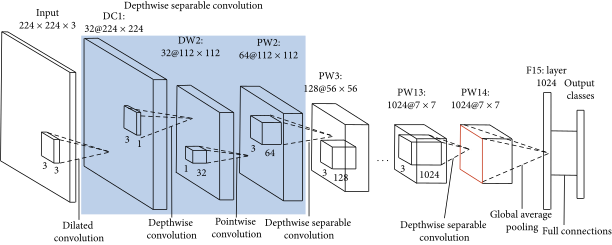
\includegraphics[height=0.27\textheight]{images/mobilenet-architecture.png}
	\caption{Architektur eines Mobilenet v2\\(Quelle: https://www.hindawi.com/journals/cin/2020/8817849/fig2/ abgerufen am 30.07.2021) }
	\label{fig:mobilenet-architecture}
\end{figure}
\section{Wiedererkennung von Objekten}
\label{sec:basics:wiedererkennung}
Das Einlernen und Wiedererkennen von Objekten ist im Bereich des Maschinelles Lernens noch heute eine Herausforderung für eingebettete beziehungsweise mobile Endgeräte, aufgrund der geringen Rechenleistung, die zur Verfügung steht. Es ist möglich diese Aufgabe mithilfe einer Cloudlösung auf einen externen leistungsstarken Server zu übertragen. Aufgrund von Nachteilen, wie beispielsweise Sicherheitsrisiken, die beim Übertragen von sensitiven Daten auftreten, wird im Rahmen dieser Arbeit eine Applikation programmiert, die den gegebenen Anwendungsfall mit der dem Endgerät zur Verfügung stehenden Hardware löst.\\
Ein naiver Ansatz, um dieses Problem lösen zu können ist ein  \ac{cnn} bei Eingang neuer Trainingsdaten erneut zu trainieren mitsamt den bereits vorhandenen Daten. Ein derart riesiger Lernvorgang ist jedoch nicht praktikabel und könnte mehrere Stunden oder sogar Tage dauern. Wenn lediglich die neuen Daten für das Training verwendet werden, resultiert dies im bekannten Phänomen des \textit{Katastrophalen Vergessen} \cite{Senchanka2019}.
\subsection{Katastrophales Vergessen}
Neuronale Netze tendieren dazu beim Einlernen von aufeinanderfolgenden unterschiedlichen Aufgaben das bereits gelernte Wissen zu vergessen. Dieses Phänomen wird als Katatrophales Vergessen beziehungsweise als \textit{Katastrophale Inferenz} bezeichnet. Die Ursache hierfür ist, dass Gewichte von Neuronen, die für eine vorherige Aufgabe wichtig sind, überschrieben werden, um die neue eingelernte Aufgabe zu erfüllen \cite{forgetting}.\\
Für den gegebenen Anwendungsfall bedeutet dies, dass alte bereits eingelernte Objekte nicht mehr erkannt werden können, wenn ein bereits trainierter Datensatz mit unbekannten Daten weitertrainiert wird. Lösungsansätze für dieses Problem werden im Folgenden erklärt.

\subsection{Transfer Learning}
Jedes menschliche Gehirn, ist dazu fähig Wissen, welches für eine Aufgabe benötigt wird, auf eine andere Aufgabe zu übertragen. So ist es beispielsweise mit geringem Aufwand möglich das Autofahren zu erlernen, wenn man bereits Motorrad fahren kann. Da es eine ähnliche Aufgabe ist, wird nicht versucht die neue Aufgabe von Grund auf neu zu lernen, sondern das Wissen, welches in der Vergangenheit erlernt werden konnte auf ein neuen ähnlichen Anwendungsfall zu transferieren.\\
Im traditionellen Ansatz des Maschinellen Lernens wird ein Datensatz aufbereitet, welcher für eine bestimmte Aufgabe zugeschnitten ist.\\
Die grundlegende Aufgabe, die in dieser Arbeit zu erfüllen ist, ist jedoch das Einlernen von neuen Trainingsdaten. Hierfür kann der Ansatz des sogenannten Transfer Learnings Anwendung finden.\\
Beim Transfer Learning wird ein bereits trainiertes \ac{ml}-Modell verwendet. Das bereits errungene Wissen kann hierbei weiterverwendet werden, um mit einem kleineren Trainingsdatensatz eine neue ähnliche Aufgabe erfüllen zu können. Erkannte Merkmale wie Formen, Kanten und Ecken können demnach durch den Wissenstransfer mit einem Modell geteilt werden. Bei dieser Vorgehensweise werden die unteren Schichten, welche die nicht-klassenspezifischen Merkmale erkennen eingefroren. Dies bedeutet, dass die Gewichte der Neuronen unveränderbar sind. Die oberen Schichten sind weiterhin trainierbar. Durch Training eines Datensatzes, welcher den neu einzulernenden Daten ähnelt, werden lediglich die klassenspezifischen Merkmale trainiert \cite{Senchanka2019}. In Abbildung \ref{fig:tf-architecture} wird diese Architektur mit dem Traditionellen \ac{ml}-Ansatz verglichen.\\
Wenn stets neue Klassen eingelernt werden sollen und diese Daten sich nicht innerhalb einer Trainingsstapels befinden, tritt jedoch das Phänomen des Katastrophalen Vergessens auf und früher eingelernte Objekte werden überschrieben \cite{cl-vs-tl}.\\
\begin{figure}[hptb]
	\centering
	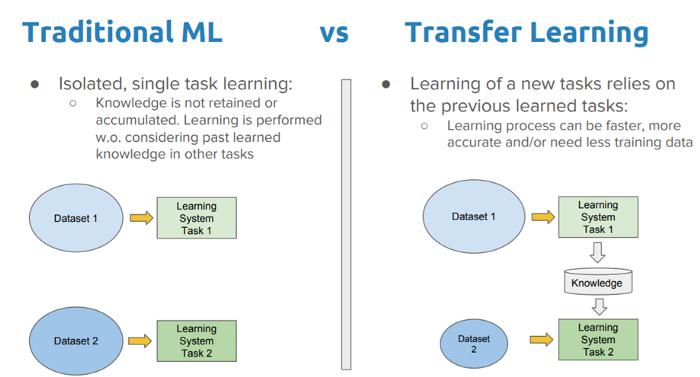
\includegraphics[height=0.4\textheight]{images/traditional-vs-tflearning.png}
	\caption{Vergleich des Aufbaus eines Transfer Learning Models im Gegensatz zum Traditionallen Maschinellen Lernens (Quelle: \cite{Sarkar2019}) }
	\label{fig:tf-architecture}
\end{figure}
\subsection{Latent-Replay-Algorithmus}
Das grundlegende Konzept beim Latent-Replay-Algorithmus bildet das sogenannte \textit{Replay} beziehungsweise \textit{Rehearsal}. Bereits trainierte Trainingsdaten werden hierfür in einem separaten Datenbank persistent gespeichert und bei Eingang neuer Trainingsdaten ebenfalls mitgelernt.
Das Problem hierbei ist jedoch, dass die Trainingsdauer massiv zunimmt, da in jeder Trainingsepoche mehrere Trainingsiterationen durch das Neuronale Netz notwendig sind. Zudem ergibt sich aus dem Abspeichern von alten Trainingsdaten ein Speicherproblem auf eingebetteten Systemen.\\
Der Latent-Replay-Algorithmus erweitert den Ansatz des Rehearsals, um eben diese Schwierigkeiten zu beheben. Hierfür werden nicht rohe Bilddaten abgespeichert sondern Aktivierungen von Neurononen innerhalb einer Schicht der Netzarchitektur. Bei einer Trainingsiteration werden neue Eingangsdaten durch Schichten des Netzen weitergeleitet, welche für das Erkennen von generischen Merkmalen zuständig sind, wie beispielsweise Ecken und Kanten. Anschließend werden diese Daten in die Latent-Replay-Schicht, welche die Speicherung der alten Trainingsdaten übernimmt, weitergeleitet, wobei die Eingangsdaten nun mit den Aktivierungen der alten Trainingsdaten vermischt werden. Die Schichten, die oberhalb der Latent-Replay-Schicht angesetzt sind, sind für die Erkennung von klassenspezifischen Merkmalen zuständig \cite{Pellegrini2019}. In Abbildung \ref{fig:latent-replay} wird der eben erklärte Aufbau dargestellt.\\
Das Prinzip des Transfer Learnings kann dementsprechend mithilfe des Latent-Replay-Algorithmus erweitert werden und dadurch das Phänomen des Katastrophalen Vergessens beheben, durch das Mittrainieren von alten Trainingsdaten.

\begin{figure}[htbp]
  \centering
  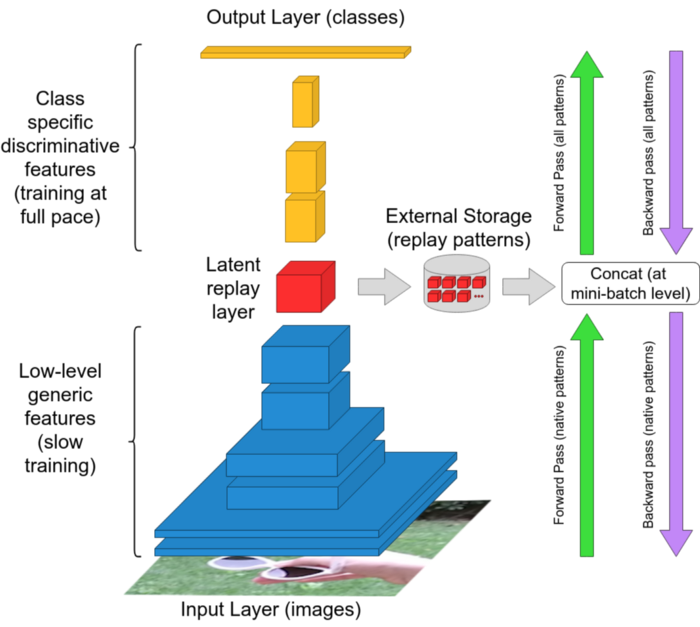
\includegraphics[height=0.5\textheight]{images/latent-replay.png}
  \caption{Architekturdiagramm des Latent Replay (Quelle: \cite{Pellegrini2019}) }
  \label{fig:latent-replay}
\end{figure}
% ---
\chapter{Anforderungsanalyse}
\label{cha:analyse}
Zur Erarbeitung der Anforderungen der gegebenen Aufgabenstellung, werden diese hinsichtlich ihrer Umsetzungsrelevanz gegliedert und gewichtet.
\begin{itemize}
\item \textbf{Must-Have-Anforderungen} sind unbedingt umzusetzen. Sie umfassen die Kernfunktionalitäten, die zur Lösung der gegebenen Aufgabenstellung essentiell sind.
\item \textbf{Should-Have-Anforderungen} beschreiben Eigenschaften des Systems, die vorteilhaft für die Lösung der gegebenen Aufgabenstellung sind und einen großen Mehrwert für die Software bieten, jedoch nicht zwingend erforderlich sind.
\item \textbf{Could-Have-Anforderungen} sind optionale Anforderungen an Eigenschaften des Systems, die ebenfalls einen relevanten Mehrwert bieten können, welcher jedoch nicht zwingend erforderlich für die Lösung der gegebenen Aufgabenstellung ist. 
\item \textbf{Nice-To-Have-Anforderungen} sind ebenfalls optionale Anforderungen an Eigenschaften des Softwaresystems. Diese sind jedoch von untergeordneter Bedeutung.
\end{itemize}
Im Folgenden werden die Anforderungen an das zu entwickelnde Softwaresystem thematisch gruppiert und unterteilt in funktionale und nicht-funktionale Anforderungen.
\section{Funktionale Anforderungen}
Funktionale Anforderungen erklären, welche Funktionen und Dienste vom Software-System bereitzustellen sind und insbesondere die Beziehungen zwischen den Ein- und Ausgabedaten.

\subsection{Lauffähigkeit als Android-App}
Eine auf einem aktuellen Android-Betriebssystem lauffähige Applikation soll entwickelt und auf einem Smartphone in den Betrieb genommen werden. Es wird gefordert, dass der Nutzer des Software-Systems die im Smartphone integrierte Kamera nutzt und diese als Eingabe für das Einlernen und die Wiedererkennung eines Objektes nutzt.  -- \textit{Gewichtung:} Must-Have-Anforderung.
\subsection{Entwicklung einer graphischen Benutzeroberfläche}
Es wird gefordert eine Graphische Benutzeroberfläche zur Verfügung zu stellen, mit welcher der Nutzer interagieren kann. Der Touchscreen des Smartphones sollte das Haupteingabegerät des Nutzers zur Steuerung der Applikation sein. -- \textit{Gewichtung:} Must-Have-Anforderung.
\subsection{Einlernen von Objekten mithilfe einer Kamera}
Es wird gefordert, dass ein Objekt mit der integrierten Smartphone-Kamera, bei guten Licht- und Kontrastverhältnissen eingelernt werden kann. Bei schlechten Licht- und Kontrastverhältnissen, die das Einlernen des Objekts erschweren oder gar technisch unmöglich machen, soll der Nutzer darauf hingewiesen werden, um mit dem Einlernen des Objektes fortfahren zu können. Bei erfolgreicher Abspeicherung der Daten, soll dem Nutzer dies mitgeteilt werden. Der Nutzer hat nun die Möglichkeit das eingelernte Objekt mit Daten zu versehen, wie beispielsweise einem Namen. Die Informationen über das nun eingelernte Objekt werden in einer Datenbank persistent abgespeichert, um sie wieder abrufen zu können. -- \textit{Gewichtung:} Must-Have-Anforderung.

\subsection{Wiedererkennung bereits eingelernter Objekte mithilfe einer Kamera}
Ein bereits eingelerntes Objekt soll bei guten Licht- und Kontrastverhältnissen vom Softwaresystem in Echtzeit wiedererkannt werden. Bei schlechten Licht- und Kontrastverhältnissen soll der Nutzer auf diese Schwierigkeiten hingewiesen werden, um diese gegebenfalls zu beheben. -- \textit{Gewichtung:} Must-Have-Anforderung.

\subsection{Markierung der wiedererkannten Objekte}
Wenn ein Objekt von der Applikation erkannt wird, soll es beispielsweise durch das Einblenden des Namens des Objektes dem Nutzer mitgeteilt werden, dass das eingelernte Objekt wieder auf dem Display des Smartphones zu sehen ist. -- \textit{Gewichtung:} Should-Have-Anforderung.
\subsection{Graphisches Overlay bei wiedererkannten Objekten}
Die beim eingelernten Objekt gespeicherten Daten sollen als ein graphisches Overlay auf dem Bildschirm des Smartphones dargestellt werden, wenn das Objekt erneut erkannt worden ist. -- \textit{Gewichtung:} Could-Have-Anforderung.
\subsection{Anbindung eines Datenbank-Servers}
Um bereits eingelernte Objekte mit anderen Nutzern teilen zu können, wird gefordert einen Datenbank-Server an die Applikation anzubinden. Ein Nutzer hat nun die Möglichkeit die Verbindung zu einem Datenbank-Server herzustellen. Dies ermöglicht es eingelernten Objekte von anderen Nutzern lokal abzuspeichern und wiederzuerkennen. -- \textit{Gewichtung:} Nice-To-Have-Anforderung.
\subsection{Nutzerprofil}
Nutzer sollten sich mit einem Namen und einem Passwort anmelden können und dadurch ihre gespeicherten Daten einsehen können. Die Nutzerdaten werden auf einem Datenbank-Server persistent abgespeichert. Die Graphische Oberfläche des Software-Systems soll einen Anmeldebildschirm zur Verfügung stellen. Wenn der Nutzer einen Nutzername und ein Passwort eingibt und seine Eingabe bestätigt sollen diese mit der Datenbank abgeglichen werden. Wenn die Anmeldedaten gespeichert sind, wird der Nutzer angemeldet. In allen anderen Fällen wird eine entsprechende Fehlermeldung ausgegeben. -- \textit{Gewichtung:} Nice-To-Have-Anforderung.
%
\section{Nicht-funktionale Anforderungen}
% Wie gut soll das System das leisten? 
Im Folgenden werden die Einschränkungen und Qualitätsmerkmale an die Entwicklung und den Betrieb des Systems erklärt.

\subsection{Lauffähigkeit auf einem Smartphone}
Die Kompatibilität und ein angemessenes Laufzeitverhalten auf einem aktuellen Android-basierten Smartphone wird gefordert, um eine benutzerfreundliche Applikation bereitstellen zu können. -- \textit{Gewichtung:} Must-Have-Anforderung.

\subsection{Dauer und Umstände des Erlernens der Objekte}
Ein Objekt soll in annehmbarer Zeit eingelernt werden. Bei schlechten Lichtverhältnissen oder anderen Umständen, die es der Technologie unmöglich macht ein Objekt einzulernen, soll der Nutzer darauf hingewiesen werden, die Lichtverhältnisse oder andere Umstände zu verbessern, um mit dem Anwenden der Applikation fortfahren zu können. -- \textit{Gewichtung:} Must-Have-Anforderung.

\subsection{Benutzerfreundlichkeit}
Die Graphische Benutzeroberfläche ist so intuitiv wie möglich zu gestalten, um die Bedienung des Systems ohne größeren Einarbeitungsaufwand erlernen zu können. -- \textit{Gewichtung:} Should-Have-Anforderung.

\subsection{Wartbarkeit und Erweiterbarkeit}
Änderungen und Erweiterungen des Software-Systems sollten mit hinnehmbarem Aufwand bewerkstelligt werden können. Demnach sollte der Quellcode modular, strukturiert und dokumentiert sein. -- \textit{Gewichtung:} Should-Have-Anforderung.

%---
\chapter{Entwurf}
\label{cha:Entwurf}
Auf der Basis der im vorangegangenen Kapitel erstellten Problemanalyse 
und der im Grundlagenkapitel aufgearbeiteten theoretischen Kenntnisse 
wird ein Lösungskonzept erarbeitet.

Bei Software-Projekten entspricht dieses Kapitel typischerweise der 
Analyse \& Design-Phase des \ac{rup}. Typische Ergebnisse dieser Phase sind 
Klassendiagramme etc.
\section{Grundlegende Designentscheidungen}
\subsection{Tensorflow Lite und Transfer Learning}
\subsection{}
\section{Grobentwurf}
Hier kommen Komponenten UMLs rein, Software Architektur
\section{Feinentwurf}
Feine UMLs über Klassen, Sequenzdiagramme, Algorithmen Flussdiagramme, Verarbeitungspipelines

%---
\chapter{Implementierung}
\label{cha:implementierung}
Transfer Learning, quantisiertes MobilenetV2, Imagenet. 

Ein Problem das beim Nutzen des Transfer Learnings aufgetreten ist, ist dass alle Trainingsdaten sich im derzeitigen Trainingsbatch befinden müssen, da sonst das Problem des Katastrophalen Vergessens aufkommt.
In diesem Kapitel wird die konkrete Implementierung des im Kapitel
\ref{cha:loesungskonzept} entwickelten Lösungskonzepts beschrieben.
Hierbei wird auf die konkret verwendeten Entwicklungswerkzeuge etc. 
Bezug genommen.

Bei Software-Projekten besteht dieses Kapitel typischerweise aus den 
Phasen Implementierung \& Test im \ac{rup}.

Zum Beispiel kann man hier auch ein kleines Listing einfügen.

\begin{lstlisting}[language=c,%
                   caption={Überschrift des Quelltexts}]
#include<stdio.h>

int main() {
    // Kommentar
    int answer = 20 << 1;
    answer += 2;
    printf("Hallöchen Welt!\n");
    printf("Die Antwort ist: %d\n", answer);
    return 0;
}
\end{lstlisting}

Manchmal hilft auch eine kleine Tabelle:

\begin{table}[htbp]
\centering
\begin{tabular}{|l|r|}
\hline
\textbf{Messwert a} & \textbf{Messwert b} \\ \hline
9 & 5 \\ \hline
1 & 4 \\ \hline
1 & 3 \\ \hline
\end{tabular}
\caption{Überschrift der Tabelle}
\label{tab:my-table}
\end{table}

Details siehe Tabelle~\ref{tab:my-table}.
%---
\chapter{Tests}
\label{cha:tests}

Aufgabe des Kapitels Inbetriebnahme ist es, die Überführung der in 
Kapitel \ref{cha:implementierung} entwickelte Lösung in das betriebliche 
Umfeld aufzuzeigen. Dabei wird beispielsweise die Inbetriebnahme eines 
Programms beschrieben oder die Integration eines erstellten 
Programmodules dargestellt.

Bei der Software-Erstellung entspricht dieses Kapitel der 
Auslieferungsphase (Deployment) im \ac{rup}.

%---
\chapter{Evaluation}
\label{cha:evaluation}
Aufgabe des Kapitels Evaluierung ist es, in wie weit die Ziele der 
Arbeit erreicht wurden. Es sollen also die erreichten Arbeitsergebnisse 
mit den Zielen verglichen werden. Ergebnis der Evaluierung kann auch 
sein, das bestimmte Ziele nicht erreicht werden konnten, wobei die 
Ursachen hierfür auch außerhalb des Verantwortungsbereichs des 
Praktikanten liegen können.

%---
\chapter{Zusammenfassung und Ausblick}
\label{cha:zusammenfassung}

\section{Erreichte Ergebnisse}
\label{sec:ergebnisse}

Die Zusammenfassung dient dazu, die wesentlichen Ergebnisse des 
Praktikums und vor allem die entwickelte Problemlösung und den 
erreichten Fortschritt darzustellen. (Sie haben Ihr Ziel erreicht und 
dies nachgewiesen).

\section{Ausblick}
\label{sec:ausblick}

Im Ausblick werden Ideen für die Weiterentwicklung der erstellten Lösung 
aufgezeigt. Der Ausblick sollte daher zeigen, dass die Ergebnisse der 
Arbeit nicht nur für die in der Arbeit identifizierten Problemstellungen 
verwendbar sind, sondern darüber hinaus erweitert sowie auf andere 
Probleme übertragen werden können.

\subsection{Erweiterbarkeit der Ergebnisse}
\label{sub:erweiterbarkeit}

Hier kann man was über die Erweiterbarkeit der Ergebnisse sagen.

\subsection{Übertragbarkeit der Ergebnisse}
\label{sub:uebertragbarkeit}

Und hier etwas über deren Übertragbarkeit.

%-----------------------------------------------------------------------
\appendix

%---
\printbibliography[heading=bibintoc]

%---
\chapter{Anhang A}

%---
\chapter{Anhang B}


\end{document}